\documentclass[12pt]{article}

\usepackage{sbc-template}
\usepackage{graphicx,url}
\usepackage[utf8]{inputenc}
\usepackage[T1]{fontenc}
\usepackage[brazil]{babel}
\usepackage{booktabs}
\usepackage{array}
\usepackage{tabularx}
\usepackage{tikz}
\usetikzlibrary{arrows.meta,positioning,shapes.geometric}
\usepackage{pdfpages}
% Compat babel/LaTeX recente
\providecommand{\normalsfcodes}{}

\sloppy
\input{links}

\title{Detecção de Imagens Sintéticas após Transformações Digitais:\\
do experimento clássico ao detector VerifAI}

\author{Nathália G. Ribas\inst{1}, Igor M. da Rosa\inst{1}}

\address{Departamento de Computação (DEC)\\
Universidade Federal de Santa Catarina\\
Araranguá, SC
\email{ribas.nathalia@grad.ufsc.br, igor.matos.rosa@grad.ufsc.br}
}

\begin{document}

\maketitle

\begin{abstract}
This report describes VerifAI, a classical computer vision detector (FFT, HOG, LBP + SVM) for AI-generated images after digital transforms. Early setups with CIFAKE, CelebA and unpaired social AI data failed to generalize. The final training set uses 5{,}000 COCO photos paired with 5{,}000 synthetic twins produced locally (image$\rightarrow$JSON$\rightarrow$AI image with ControlNet). On a 4{,}000/1{,}000 pair holdout, fusion reaches 88.15\% accuracy. A Streamlit app scores the whole letterboxed image. Limitations of SVM versus deep learning for open-world images are discussed.
\end{abstract}

\begin{resumo}
Este relatório descreve o VerifAI, detector clássico (FFT, HOG, LBP + SVM) para imagens geradas por IA após transformações digitais. Configurações iniciais com CIFAKE, CelebA e bases de IA de rede sem REAL proporcional falharam na prática. A base final usa 5{.}000 fotos COCO pareadas a 5{.}000 versões sintéticas geradas localmente (imagem$\rightarrow$JSON$\rightarrow$imagem IA com ControlNet). No holdout 4{.}000/1{.}000 pares, a fusão atinge 88,15\% de acurácia. Um app Streamlit avalia a imagem inteira (letterbox 224). Discutem-se também as limitações do SVM frente a deep learning em imagens fora do domínio treinado.
\end{resumo}

% Capa (título + resumos) fica sozinha; sumário na página seguinte
\newpage
\setcounter{tocdepth}{1}
\tableofcontents
\newpage

%----------------------------------------------------------------------
\section{Introdução}
%----------------------------------------------------------------------

Imagens geradas por inteligência artificial circulam em redes sociais, campanhas eleitorais, anúncios de imóveis e mensagens instantâneas. Quase nunca chegam intactas: passam por compressão JPEG, recorte, redimensionamento e filtros. Detectores que acertam a foto ``limpa'' podem falhar depois dessas mudanças --- comportamento observado em testes exploratórios com o ZeroGPT\footnote{\url{https://www.zerogpt.com/pt/ai-image-detector}} (Figura~\ref{fig:zerogpt}).

\begin{figure}[ht]
\centering
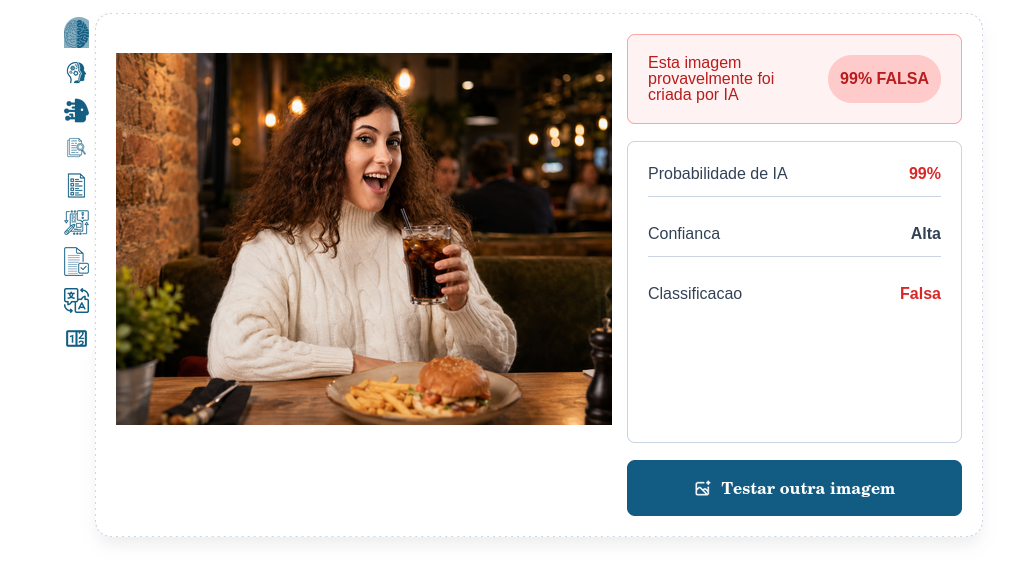
\includegraphics[width=0.48\textwidth]{suporte/TestePosTransformacao.png}
\hfill
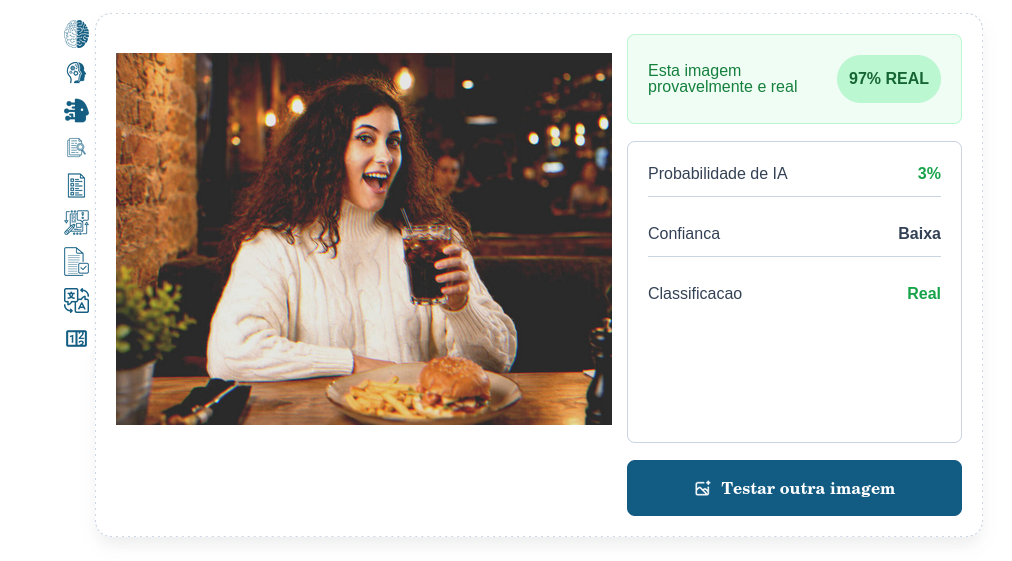
\includegraphics[width=0.48\textwidth]{suporte/TesteReducaoReso.png}
\caption{Motivação com ZeroGPT. À esquerda: cena alterada por IA marcada como falsa. À direita: após compressão, o mesmo conteúdo é tratado como real.}
\label{fig:zerogpt}
\end{figure}

A pergunta central do trabalho é: \emph{quão robustos são detectores baseados em features clássicas quando a imagem sofre transformações típicas da internet?} Ao longo do projeto, essa pergunta se desdobrou em duas outras, igualmente práticas. Em primeiro lugar, qual base de treino realmente serve para um aplicativo? Bases famosas --- CIFAKE, CelebA e coleções de IA coletadas em redes --- mostraram acurácia enganosa no laboratório e falharam no uso real, como se discute na Seção~\ref{sec:bases}. Em segundo lugar, como alinhar as classes REAL e FAKE? Sem o par inverso (mesma cena e mesma pose), o classificador tende a aprender o assunto da foto, e não o artefato de síntese.

A solução desenvolvida, denominada \textbf{VerifAI}, combina visão computacional clássica e um protocolo de dados alinhado ao uso do detector. A imagem é descrita por três famílias de descritores --- FFT no domínio da frequência, HOG no domínio espacial e LBP no domínio da textura --- cuja concatenação alimenta uma máquina de vetores de suporte com kernel RBF~\cite{cortes1995svm,dalal2005hog,ojala2002lbp,gonzalez2018}. O treino inclui um aumento de dados \emph{leve} (compressão JPEG, redimensionamento, suavização e um pipeline combinado), de modo que o classificador veja, já na aprendizagem, degradações próximas às da internet, sem destruir o sinal espectral necessário à FFT. A base de treino é \textbf{pareada}: cada foto real do COCO~\cite{coco2017} possui uma gêmea sintética gerada localmente pelo fluxo imagem$\rightarrow$JSON$\rightarrow$imagem IA, com Stable Diffusion~1.5 e ControlNet Depth, preservando geometria e composição. Por fim, a interface Streamlit avalia a \textbf{imagem inteira} encaixada em $224{\times}224$ (letterbox), alinhando inferência e treino e evitando o grid de janelas herdado de experimentos em $32{\times}32$.

\subsection{Objetivos e contribuições}

Os objetivos do trabalho foram: (i)~medir a queda de desempenho após transformações digitais típicas (JPEG, crop, resize, blur e pipeline combinado); (ii)~construir uma base REAL/FAKE proporcional e alinhada em cena e pose, adequada a um detector de aplicativo; (iii)~entregar um classificador clássico interpretável --- fusão de features com SVM --- e uma interface de inspeção; e (iv)~documentar o que não funcionou nas bases anteriores e por quê.

As contribuições resultantes incluem o diagnóstico das bases desalinhadas (CIFAKE, CelebA e Harvard AIGI cruzado com COCO), o pipeline local e retomável COCO$\rightarrow$JSON$\rightarrow$IA com BLIP, Stable Diffusion~1.5 e ControlNet Depth (5{.}000 pares), o detector calibrado com 88,15\% de acurácia no holdout 4{.}000/1{.}000, o aplicativo VerifAI com zona inconclusiva e scores auxiliares, e a discussão explícita dos limites do SVM fora do domínio treinado frente à alternativa de deep learning. Links oficiais constam da Seção~\ref{sec:links}; o poster integra o Anexo~\ref{anexo:poster}.

%----------------------------------------------------------------------
\section{Trabalhos relacionados}
%----------------------------------------------------------------------

Bird e Lotfi~\cite{bird2024cifake} propuseram o CIFAKE --- imagens reais do CIFAR-10 e sintéticas geradas com Stable Diffusion, todas em $32{\times}32$ --- e reportaram cerca de 93\% de acurácia com CNN. O conjunto é balanceado e já foi usado com features manuais~\cite{nirob2026handcrafted}, o que motivou os primeiros experimentos deste projeto. Contudo, a resolução baixa e o domínio fechado do CIFAR-10 limitam a transferência para fotos de celular em resolução nativa.

Frank et al.~\cite{frank2020frequency} mostraram que GANs deixam marcas no espectro de frequência ligadas ao \emph{upsampling}. Bammey~\cite{bammey2024synthbuster} estendeu a ideia a modelos de difusão (Synthbuster), reforçando o uso de FFT e o teste sob JPEG. Nirob et al.~\cite{nirob2026handcrafted} compararam histograma, DCT, HOG, LBP, GLCM e wavelets com classificadores clássicos; a fusão de descritores manuais melhorou o desempenho. Choi et al.~\cite{choi2025warpad} evidenciaram que crop e resize prejudicam detectores, alinhando-se ao foco em robustez.

No domínio de dados abertos, o Microsoft COCO~\cite{coco2017} oferece fotos diversas (pessoas, objetos, cenas urbanas e naturais). Já coleções de imagens sintéticas coletadas em redes sociais~\cite{harvardAIGI} concentram FAKE ``em produção'', porém sem um REAL proporcional do mesmo universo visual --- lacuna que se mostrou crítica nos experimentos deste relatório.

O presente trabalho mantém a linha clássica (FFT/HOG/LBP + SVM)~\cite{gonzalez2018,dalal2005hog,ojala2002lbp,cortes1995svm}, mas desloca o eixo para \emph{domínio alinhado} entre REAL e FAKE e para um aplicativo de inspeção (VerifAI), em vez de se limitar ao CIFAKE em baixa resolução. A geração local de gêmeas sintéticas com ControlNet Depth é o elo que faltava entre a literatura de frequência e o uso prático do detector.

%----------------------------------------------------------------------
\section{Fundamentação}
\label{sec:fundamentacao}
%----------------------------------------------------------------------

\subsection{Visão clássica versus aprendizado profundo}

Há dois caminhos principais para decidir se uma imagem é real ou gerada por IA. Na \emph{visão clássica}, a imagem é resumida por descritores calculados explicitamente --- frequência, bordas e textura --- e um classificador, tipicamente SVM, aprende a fronteira entre as classes~\cite{gonzalez2018,nirob2026handcrafted}. Cada componente do vetor tem interpretação visual, o que permite relacionar uma transformação (JPEG, crop, blur) à degradação de um domínio específico.

No \emph{aprendizado profundo}, uma rede convolucional ou um \emph{backbone} moderno aprende os padrões internamente. No CIFAKE, esse tipo de modelo atinge cerca de 93\% de acurácia~\cite{bird2024cifake}. A contrapartida é a menor transparência e, em geral, a necessidade de mais dados e GPU para treino estável em domínio aberto. Como o escopo deste trabalho priorizou interpretabilidade e um pipeline clássico reproduzível, adotou-se a via de features manuais com SVM. A Seção~\ref{sec:discussao} discute por que um modelo profundo seria o próximo passo natural para imagens totalmente fora da base treinada.

\subsection{FFT (domínio da frequência)}

Uma imagem pode ser vista como soma de ondas de diferentes frequências~\cite{gonzalez2018}. A Transformada Rápida de Fourier (FFT) decompõe essa soma. O espectro de magnitude indica a contribuição de cada frequência: o centro concentra variações suaves (baixa frequência) e as bordas, detalhes e ruído (alta frequência).

Na detecção de conteúdo sintético, o processo de geração --- em especial o \emph{upsampling} de GANs e de modelos de difusão --- deixa marcas periódicas no espectro~\cite{frank2020frequency,bammey2024synthbuster}. A compressão JPEG também atua em frequência, ao descartar coeficientes de alta frequência. Operacionalmente, aplica-se a FFT~2D à imagem em escala de cinza, desloca-se o espectro (\texttt{fftshift}), toma-se a magnitude em escala logarítmica e reduz-se o mapa 2D a um perfil radial em 64 anéis. Acrescentam-se três razões de energia (baixa, média e alta frequência) e o centróide espectral, totalizando 68 dimensões. Não se aplica normalização min-max por imagem, a fim de preservar diferenças absolutas de energia de alta frequência entre REAL e IA.

\subsection{HOG (domínio do espaço)}

O Histograma de Gradientes Orientados (HOG) descreve a forma local da imagem~\cite{dalal2005hog}. Em cada célula, acumulam-se orientações de bordas; a concatenação dos histogramas resume o desenho da cena. No pipeline final, a imagem letterbox $224{\times}224$ é redimensionada a $128{\times}128$ para o HOG, com células $16{\times}16$ e blocos $2{\times}2$, gerando um vetor de 1{.}568 dimensões. Crop e resize alteram a geometria das bordas; o blur as suaviza. Por isso o HOG é o descritor natural para observar o efeito dessas transformações sobre a estrutura espacial da cena.

\subsection{LBP (domínio da textura)}

O Padrão Binário Local (LBP) compara cada pixel com os vizinhos em um círculo~\cite{ojala2002lbp}. Na versão uniforme ($P{=}8$, $R{=}1$), o histograma possui 10 bins. Compressão e blur alteram a relação entre um pixel e sua vizinhança; espera-se, portanto, degradação sob JPEG forte e sob suavização. O vetor curto complementa FFT e HOG sem inflar demasiadamente a dimensão da fusão.

\subsection{Fusão e SVM}

A fusão concatena os três vetores já padronizados por família (\texttt{StandardScaler}) e alimenta um SVM com kernel RBF~\cite{cortes1995svm}. A Tabela~\ref{tab:dims} resume as dimensões. Os parâmetros $C{=}10$ e $\gamma{=}\mathrm{auto}$ foram fixados após calibração. Atribui-se peso maior à classe REAL para reduzir falso positivo no aplicativo. O treino emprega ThunderSVM na GPU, com fallback \texttt{sklearn} em CPU.

\begin{table}[ht]
\centering
\small
\caption{Dimensões dos descritores no pipeline v3.}
\label{tab:dims}
\begin{tabular}{lrl}
\toprule
Descritor & Dimensão & Observação \\
\midrule
FFT   & 68    & 64 anéis + 3 bandas + centróide \\
HOG   & 1{.}568 & letterbox interno $128{\times}128$ \\
LBP   & 10    & uniforme $P{=}8$, $R{=}1$ \\
Fusão & 1{.}646 & concatenação padronizada \\
\bottomrule
\end{tabular}
\end{table}

\subsection{Pré-processamento: letterbox 224}

Diferente do CIFAKE ($32{\times}32$), o pipeline final encaixa a foto inteira em $224{\times}224$ mantendo a proporção. A borda usa reflexão (\texttt{BORDER\_REFLECT\_101}), e não preenchimento preto: bordas pretas criavam anéis artificiais no espectro FFT e empurravam a acurácia para perto do acaso. O HOG opera sobre uma resolução interna de $128{\times}128$. Com isso, o classificador observa a cena completa, alinhando treino e inferência do aplicativo.

\subsection{Transformações digitais}

No treino empregam-se seis variantes leves da mesma imagem: a original; compressões JPEG com qualidade 90 e 70; redimensionamento para a metade da resolução; suavização gaussiana $3{\times}3$; e um \emph{pipeline} que combina crop de 25\%, resize $0{,}5$ e JPEG~70. Essas variantes simulam o que ocorre quando a foto circula na internet, sem destruir por completo o sinal que a FFT precisa aprender.

Na avaliação de robustez, o catálogo inclui ainda JPEG~50 e crops de 10\%, 25\% e 40\%. Crops agressivos e JPEG~50 não entram no treino: experimentos anteriores mostraram que aumentos excessivamente pesados destroem o sinal espectral e degradam o descritor de frequência.

%----------------------------------------------------------------------
\section{Evolução das bases (o que não funcionou)}
\label{sec:bases}
%----------------------------------------------------------------------

Várias bases foram tentadas antes da solução final. O padrão comum de fracasso foi o \textbf{domínio desalinhado}: o classificador aprendia diferenças de conteúdo --- rostos versus paisagem, $32{\times}32$ versus foto de celular --- e não artefatos de síntese. A Tabela~\ref{tab:bases} resume o panorama; as subseções a seguir detalham cada tentativa.

\subsection{CIFAKE}

O CIFAKE~\cite{bird2024cifake} permitiu validar o pipeline clássico com rapidez. Treinar somente nas imagens originais alcançou cerca de 92\% de fusão no teste limpo, porém a acurácia colapsou para cerca de 54\% após crop, blur ou pipeline --- o mesmo tipo de falha observado no ZeroGPT. Incluir transformações no treino recuperou robustez, com fusão acima de 71\% após o pipeline combinado. Ainda assim, duas barreiras permaneceram para o aplicativo: a resolução forçada a $32{\times}32$ e o domínio CIFAR-10, muito diferente de fotos reais de alta resolução.

\subsection{CelebA e fotos gerais}

Usar CelebA apenas como REAL --- rostos de celebridades --- produziu muitos falsos positivos em fotos gerais: parque, corpo inteiro, rua e objetos. O SVM associava ``rosto de estúdio'' à classe REAL e tratava cenas cotidianas como suspeitas. Sem FAKE proporcional do mesmo domínio, a base mostrou-se inadequada para um detector genérico.

\subsection{Harvard AIGI e cruzamento com COCO}

A coleção Harvard AIGI~\cite{harvardAIGI} concentra imagens de IA coletadas em Instagram e Twitter/X. Treinar somente com esse FAKE, sem REAL do mesmo universo, não fecha o problema. O cruzamento COCO (REAL diverso) com Harvard (FAKE de rede) levou a FFT perto do acaso ($\sim$53\%): os domínios são diferentes demais e o classificador não encontra um eixo estável de síntese.

\subsection{Síntese da lição}

\begin{table}[ht]
\centering
\small
\caption{Bases experimentadas e motivo do abandono no detector do app.
Referências: CIFAKE~\cite{bird2024cifake}, Harvard AIGI~\cite{harvardAIGI}, COCO~\cite{coco2017}.}
\label{tab:bases}
\renewcommand{\arraystretch}{1.25}
\begin{tabular}{@{}p{2.8cm}p{3.6cm}p{6.0cm}@{}}
\toprule
\textbf{Base} & \textbf{Papel} & \textbf{Problema} \\
\midrule
CIFAKE
  & REAL/FAKE $32{\times}32$
  & Resolução baixa; falha no app com foto real \\
CelebA
  & Só rostos (REAL)
  & Muitos falsos positivos em fotos gerais \\
Harvard AIGI
  & Só FAKE de rede
  & Sem REAL proporcional do mesmo universo \\
COCO $\times$ Harvard
  & REAL + FAKE misturados
  & Domínios diferentes; FFT perto do acaso ($\sim$53\%) \\
\textbf{Pares COCO$\rightarrow$IA}
  & 5k + 5k alinhados
  & Base final adotada no VerifAI \\
\bottomrule
\end{tabular}
\end{table}

A lição prática é direta: para o aplicativo, REAL e FAKE precisam ser o \textbf{par inverso} --- mesma cena e mesma pose ---; caso contrário, o SVM decide pelo assunto da foto, e não pelo artefato de geração.

%----------------------------------------------------------------------
\section{Solução final}
\label{sec:solucao}
%----------------------------------------------------------------------

\subsection{Geração de pares: COCO $\rightarrow$ JSON $\rightarrow$ imagem IA}

A partir de 5{.}000 fotos COCO~\cite{coco2017} armazenadas em \texttt{base/landscape\_real/} --- amostra aleatória de imagens íntegras do \texttt{train2017} --- gerou-se uma gêmea sintética para cada fotografia. O fluxo, ilustrado na Figura~\ref{fig:pipeline-pares}, tem três etapas. Primeiro, o modelo BLIP (\texttt{Salesforce/blip-image-captioning-large}) descreve a cena e monta o prompt textual (imagem$\rightarrow$JSON). Em seguida, Stable Diffusion~1.5 associado ao ControlNet Depth (\texttt{lllyasviel/sd-controlnet-depth}), com estimativa de profundidade MiDaS, gera a imagem sintética mantendo a geometria --- pose e composição --- e alterando a aparência (JSON$\rightarrow$IA). Por fim, cada arquivo é salvo em \texttt{base/pares\_ia/} com o mesmo nome (\emph{stem}) da foto real correspondente, o que garante o pareamento automático no carregador de dados.

O processo foi executado localmente por um pipeline retomável (\texttt{cod/pares/}), cujo estado permanece em \texttt{base/pares\_estado.json}: se a geração fosse interrompida, a retomada continuava do último índice pendente. A Figura~\ref{fig:par} mostra um exemplo do resultado: à esquerda a foto real e à direita a versão sintética com pose correspondente. O pacote das bases (REAL e pares IA) está disponível no Drive (Seção~\ref{sec:links}).

\begin{figure}[ht]
\centering
\begin{tikzpicture}[
  node distance=0.7cm and 0.6cm,
  box/.style={draw, rounded corners, align=center, font=\small, inner sep=5pt, minimum width=2.6cm},
  arr/.style={-{Latex}, thick}
]
  \node[box, fill=blue!10] (r) {Foto REAL\\(COCO)};
  \node[box, right=of r, fill=yellow!15] (j) {JSON / prompt\\(BLIP)};
  \node[box, right=of j, fill=orange!15] (a) {Imagem IA\\(+ Depth)};
  \node[box, below=1.1cm of j, fill=green!12] (p) {Par de treino\\mesmo stem};
  \draw[arr] (r) -- (j);
  \draw[arr] (j) -- (a);
  \draw[arr] (r) |- (p);
  \draw[arr] (a) |- (p);
\end{tikzpicture}
\caption{Pipeline de geração dos pares usados no treino final.}
\label{fig:pipeline-pares}
\end{figure}

\begin{figure}[ht]
\centering
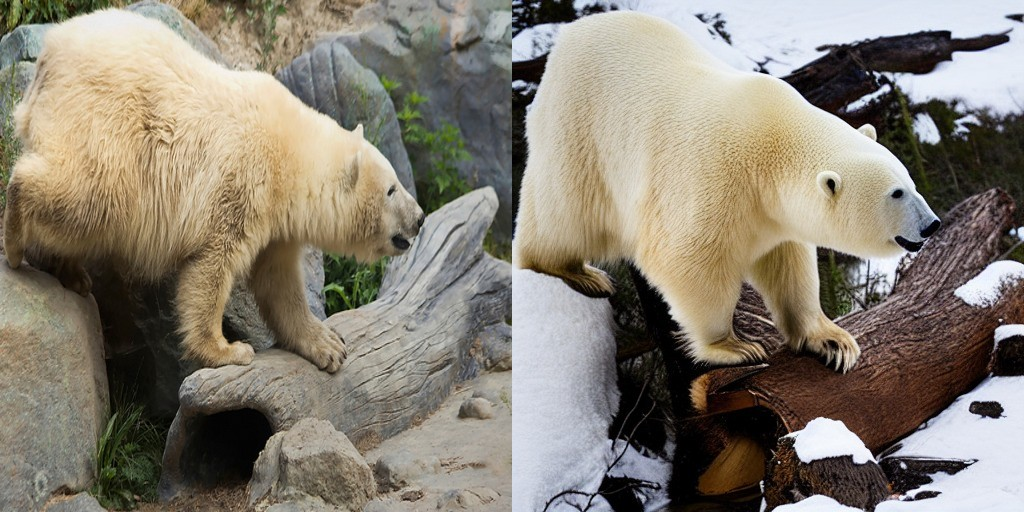
\includegraphics[width=0.95\textwidth]{suporte/par_real_ia.jpg}
\caption{Exemplo de par REAL (esquerda) $\times$ IA (direita) gerado para a base final.}
\label{fig:par}
\end{figure}

\subsection{Protocolo de treino}

O notebook \texttt{cod/main\_v3.ipynb} opera no protocolo de avaliação com 4{.}000 pares no treino (8{.}000 imagens, REAL e IA) e 1{.}000 pares no teste holdout (2{.}000 imagens), nunca vistos durante a aprendizagem. A divisão é feita por \emph{par}: o mesmo \emph{stem} não aparece nos dois lados, e a semente é fixa para reprodutibilidade. Cada imagem gera seis amostras de treino --- as variantes digitais descritas na Seção~\ref{sec:fundamentacao} --- totalizando cerca de 48{.}000 vetores por família de feature. O SVM é treinado com ThunderSVM na GPU e peso maior na classe REAL. Os artefatos persistidos são \texttt{cod/models/svm\_v3\_*.pkl} e \texttt{scaler\_v3\_*.pkl}.

\subsection{Aplicação Streamlit (VerifAI)}

O aplicativo (\texttt{app.py}, acionado por \texttt{./run\_app.sh}) foi desenhado para espelhar o treino. O usuário envia uma imagem JPEG ou PNG; aplica-se o mesmo letterbox $224{\times}224$ com borda refletida; recalculam-se FFT, HOG e LBP, cada vetor padronizado com o scaler salvo na aprendizagem; e o SVM de fusão devolve a probabilidade de a imagem ser sintética. Os scores de FFT e HOG aparecem como apoio à interpretação. Faixas de baixa chance de IA indicam provável REAL; faixas altas, provável IA; e a zona entre 40\% e 60\% é tratada como inconclusiva. Não há grid de janelas: a entrada é a imagem inteira. Os modelos são carregados de \texttt{cod/models/}.

Para inspeção manual, a pasta \texttt{base/teste\_app/} contém cinco pares (REAL e IA) nas seis variantes de treino, acompanhados de um manifesto JSON. As Figuras~\ref{fig:ex-real} e~\ref{fig:ex-ia} ilustram saídas típicas do aplicativo.

\begin{figure}[ht]
\centering
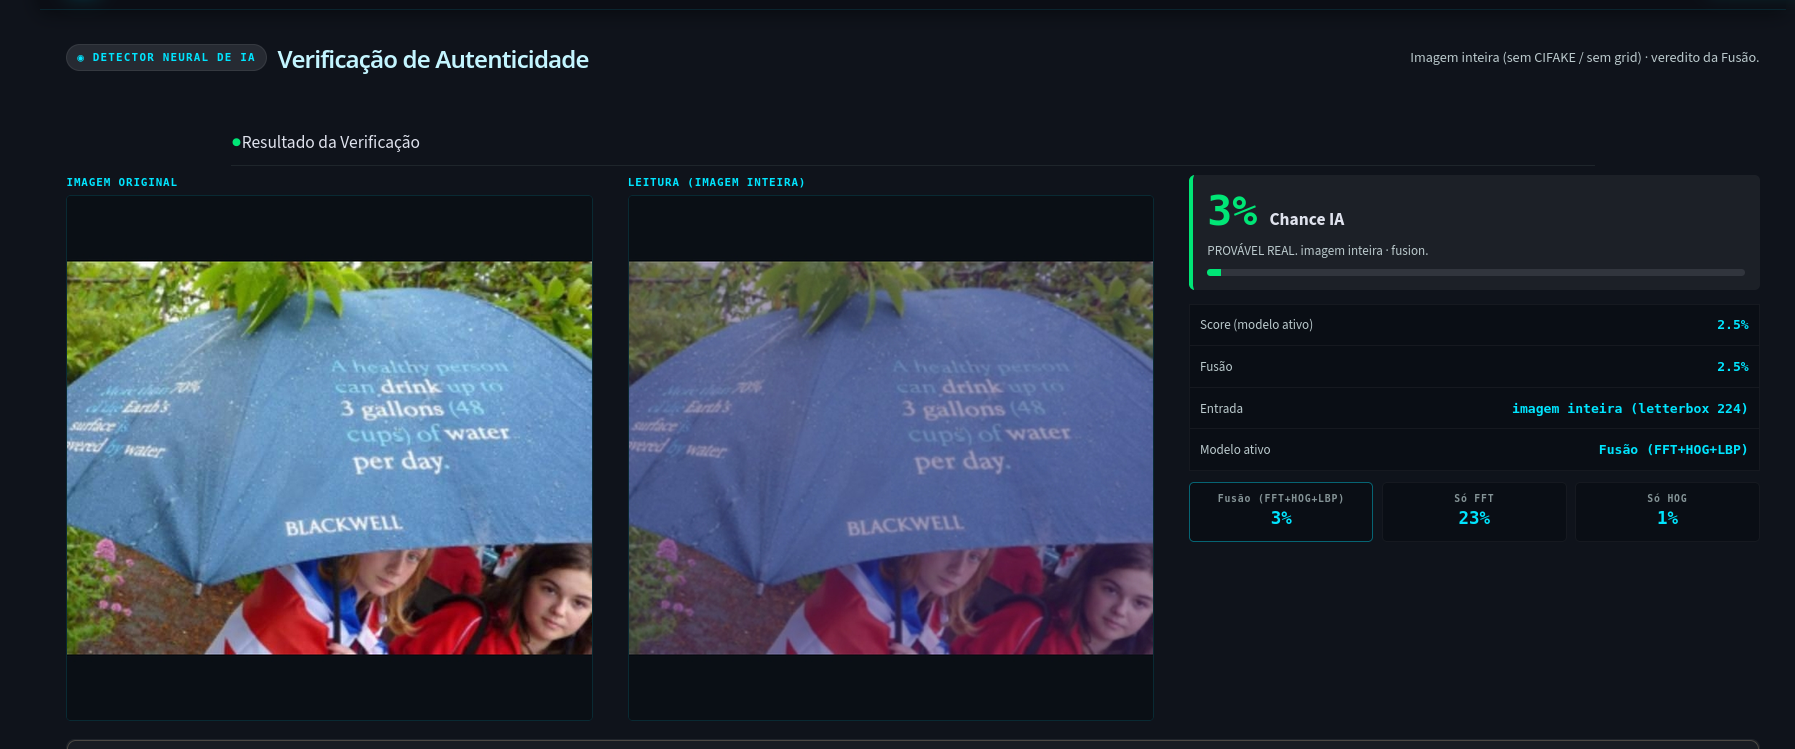
\includegraphics[width=\textwidth]{suporte/ExReal.png}
\caption{Exemplo no app: foto real classificada como provável real (baixa chance de IA).}
\label{fig:ex-real}
\end{figure}

\begin{figure}[ht]
\centering
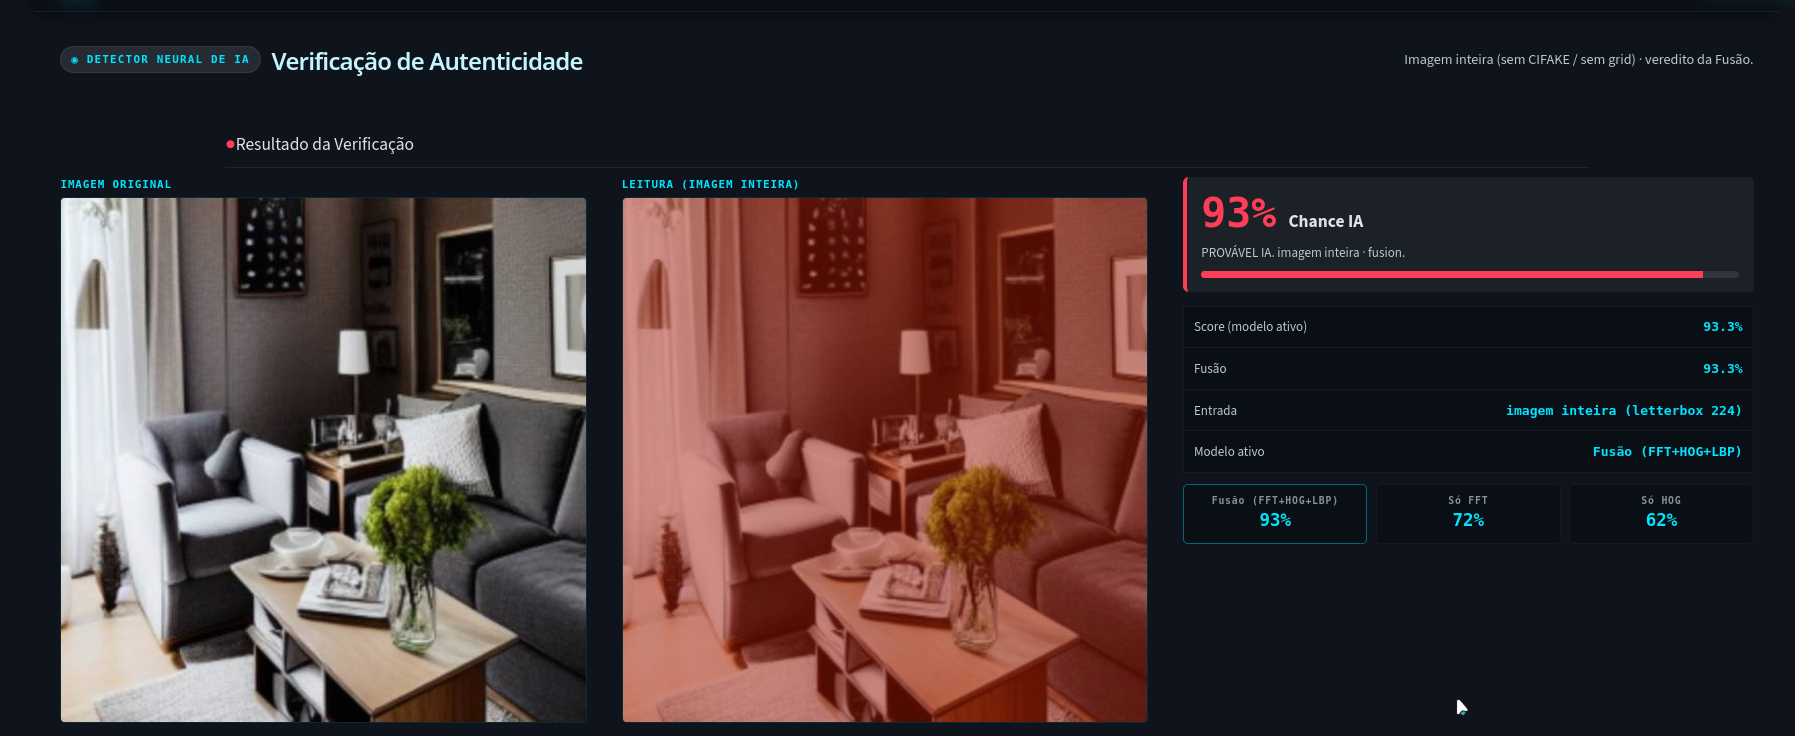
\includegraphics[width=\textwidth]{suporte/ExIA.png}
\caption{Exemplo no app: imagem sintética classificada como provável IA (alta chance de IA).}
\label{fig:ex-ia}
\end{figure}

%----------------------------------------------------------------------
\section{Resultados}
\label{sec:resultados}
%----------------------------------------------------------------------

No protocolo 4{.}000/1{.}000 pares, com aumento de dados $\times$6, a Tabela~\ref{tab:v3} resume o holdout. A fusão --- detector efetivamente usado no aplicativo --- atinge 88,15\% de acurácia. HOG (84,40\%) e LBP (82,30\%) superam a FFT isolada (75,00\%) neste domínio; a concatenação obtém o melhor equilíbrio entre precisão na classe FAKE e recall na classe REAL.

\begin{table}[ht]
\centering
\caption{Acurácia no holdout de pares (4{.}000 treino / 1{.}000 teste). SVM RBF.}
\label{tab:v3}
\begin{tabular}{lrrr}
\toprule
Feature & Acurácia & Prec.\ FAKE & Rec.\ REAL \\
\midrule
FFT    & 0,7500 & 0,799 & 0,832 \\
HOG    & 0,8440 & 0,887 & 0,899 \\
LBP    & 0,8230 & 0,860 & 0,874 \\
\textbf{Fusão} & \textbf{0,8815} & 0,865 & 0,859 \\
\bottomrule
\end{tabular}
\end{table}

\subsection{Robustez às transformações}

A Figura~\ref{fig:rob-v3} e a Tabela~\ref{tab:rob} mostram a acurácia por transformação no mesmo holdout. JPEG leve, resize e blur preservam bem a fusão, tipicamente acima de 87\%. Crops agressivos e o pipeline combinado provocam a maior queda --- a fusão cai para 74,50\% no crop de 40\% e para 79,55\% no pipeline --- ainda assim permanecendo bem acima do acaso. O mapa da Figura~\ref{fig:heat-v3} confirma que a FFT é a família mais sensível a crop e a compressão forte, enquanto HOG e a fusão absorvem melhor parte dessas degradações.

\begin{figure}[ht]
\centering
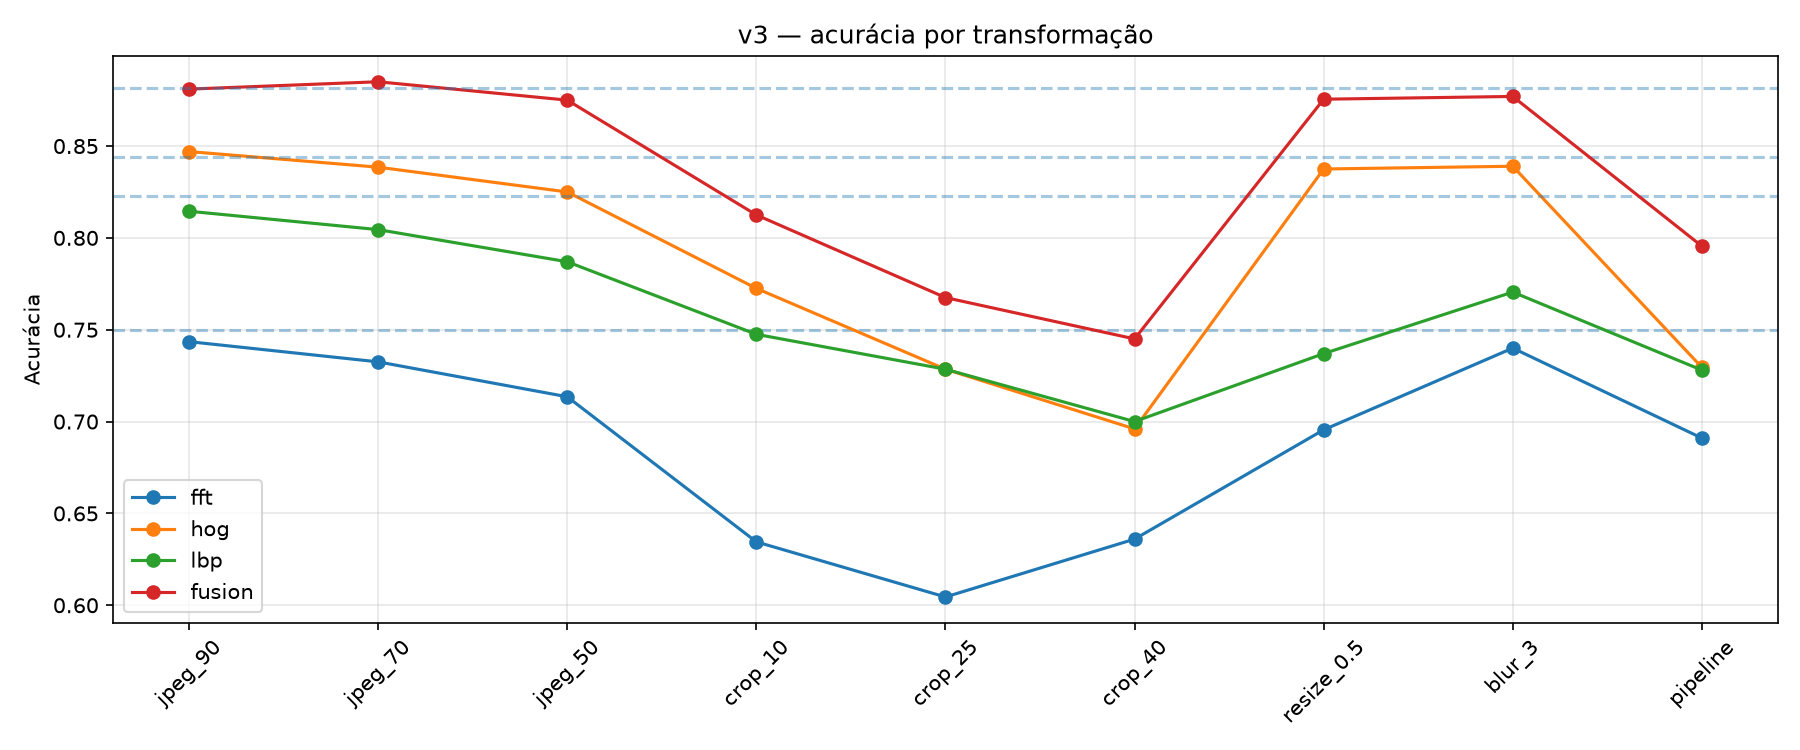
\includegraphics[width=\textwidth]{suporte/v3_acc_por_transf.png}
\caption{Acurácia por transformação no holdout v3 (pares).}
\label{fig:rob-v3}
\end{figure}

\begin{table}[ht]
\centering
\small
\caption{Acurácia da fusão por transformação no holdout (baseline 0,8815).}
\label{tab:rob}
\begin{tabular}{lrr}
\toprule
Transformação & Acurácia fusão & Queda \\
\midrule
JPEG 90      & 0,8810 & 0,0005 \\
JPEG 70      & 0,8850 & $-$0,0035 \\
JPEG 50      & 0,8750 & 0,0065 \\
Resize $0{,}5$ & 0,8755 & 0,0060 \\
Blur $3{\times}3$ & 0,8770 & 0,0045 \\
Crop 10\%    & 0,8125 & 0,0690 \\
Crop 25\%    & 0,7675 & 0,1140 \\
Crop 40\%    & 0,7450 & 0,1365 \\
Pipeline     & 0,7955 & 0,0860 \\
\bottomrule
\end{tabular}
\end{table}

\begin{figure}[ht]
\centering
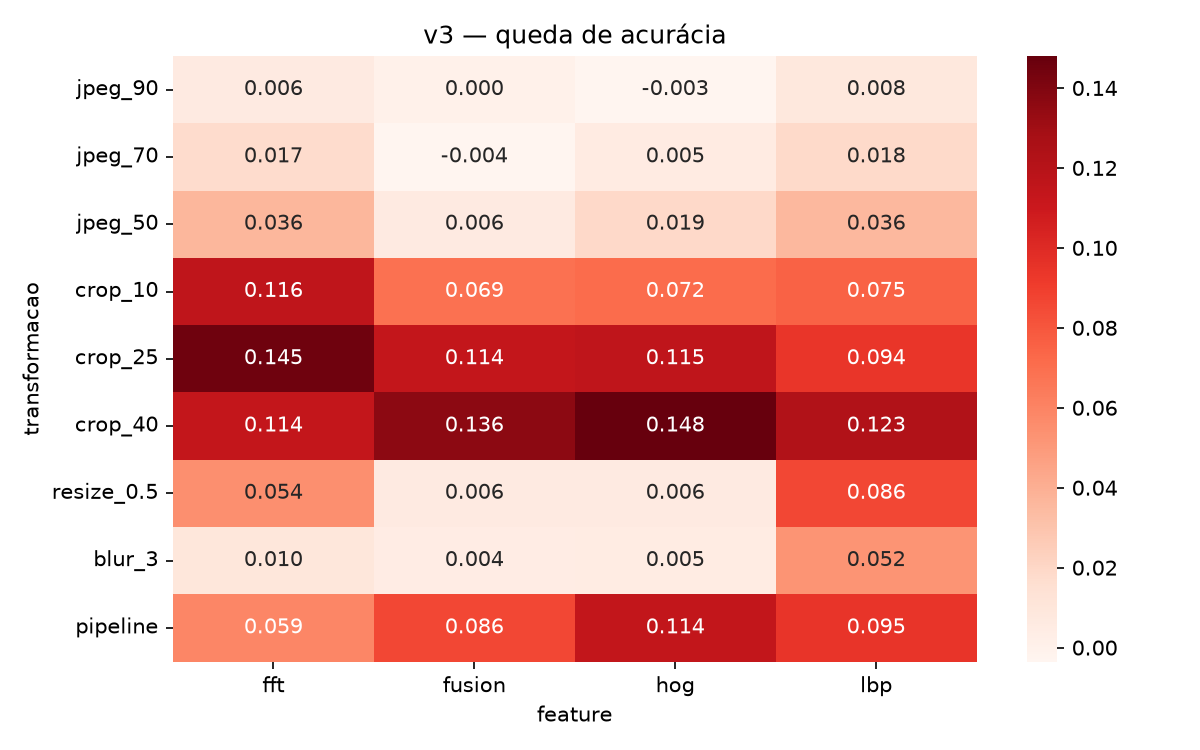
\includegraphics[width=0.92\textwidth]{suporte/v3_heatmap_queda.png}
\caption{Mapa de queda de acurácia por feature e transformação (holdout v3).}
\label{fig:heat-v3}
\end{figure}

Em comparação com o CIFAKE ``limpo'' antigo --- cerca de 92\% no original, com colapso após crop ou blur --- e com o cruzamento Harvard$\times$COCO --- cerca de 53\% na FFT ---, a base pareada recupera precisão e alinhamento com o uso real do aplicativo, desde que a imagem de teste esteja relacionada ao universo treinado (COCO ou mesma família de gerador).

%----------------------------------------------------------------------
\section{Discussão}
\label{sec:discussao}
%----------------------------------------------------------------------

Os resultados reforçam pontos práticos para um detector voltado a aplicativo e, ao mesmo tempo, deixam claras as fronteiras do desenho atual.

\subsection{O que funcionou}

A experiência com as bases anteriores mostrou que o domínio importa mais do que o volume. Dezenas de milhares de imagens FAKE de Instagram ou Twitter, sem um REAL proporcional do mesmo universo visual, pioraram o aplicativo: a FFT chegou perto do acaso ($\sim$53\%). O volume sozinho não corrige desalinhamento semântico.

Os pares gerados com ControlNet ensinam a distinção ``mesma cena, aparência sintética''. A fusão (88,15\%) supera a FFT isolada (75\%), sugerindo que HOG e LBP complementam o espectro quando a geometria da cena é compartilhada entre as classes. O aumento leve no treino prepara o modelo para JPEG, resize e blur sem destruir o sinal espectral; crops agressivos e JPEG~50 ficam reservados ao teste de robustez --- opção adotada após a FFT colapsar com aumentos excessivamente pesados. Por fim, o letterbox 224 permite usar a foto completa no aplicativo, alinhando treino e inferência, e o grid $32{\times}32$ herdado do CIFAKE foi abandonado.

\subsection{Limitações do SVM e papel do deep learning}

Um modelo com SVM sobre features fixas tem limites estruturais. O descritor FFT/HOG/LBP é uma compressão elaborada pelo projetista: captura padrões antecipados, mas não inventa representações novas quando o estilo visual muda. Em domínio aberto --- fotos de outros sensores, outros geradores (Midjourney, Flux, SDXL), selfies fortes, ilustrações ou prints de tela --- o SVM já perde bastante precisão e deixa de separar REAL de IA de forma confiável. Esse comportamento foi observado em inspeções manuais no aplicativo com imagens totalmente diferentes das treinadas: o veredito oscila, a faixa inconclusiva aparece com frequência e, em vários casos, REAL e IA se confundem.

Em contraste, um modelo de deep learning --- CNN ou \emph{transformer} de visão --- aprenderia filtros diretamente dos pixels e, com dados suficientes e diversificados, tenderia a abranger mais estilos e resoluções. A literatura de detecção de mídia sintética aponta na mesma direção: features manuais foram o ponto de partida histórico, mas representações aprendidas passaram a dominar quando o objetivo é generalizar entre geradores e plataformas~\cite{bird2024cifake}. O custo, no contexto deste trabalho, seria maior demanda de GPU, menor interpretabilidade imediata por domínio (frequência versus textura) e um ciclo de treino mais longo.

Para o escopo adotado --- interpretabilidade e entrega de um aplicativo clássico --- o SVM foi a escolha adequada. Para um detector de propósito geral, capaz de cobrir imagens bem mais diversas do que a base COCO pareada, deep learning é o caminho natural de evolução. Vale notar que mesmo detectores profundos sofrem queda fora do domínio de treino; a diferença é de grau e de capacidade de absorver diversidade quando há dados e aumento adequados. O SVM, por construção, satura mais cedo nesse eixo.

\subsection{Onde a precisão permanece alta}

Apesar da fragilidade fora do domínio, o VerifAI obtém precisão elevada quando a imagem está relacionada à base treinada --- exatamente o cenário proposto no início do projeto. Isso inclui outras fotos COCO (mesmo universo visual do REAL de treino), imagens geradas pela mesma família de IA (Stable Diffusion com condicionamento semelhante ao ControlNet Depth) e as transformações digitais do escopo inicial (JPEG, resize, blur e pipeline), conforme a Tabela~\ref{tab:rob}: a fusão permanece tipicamente acima de 87\% em JPEG, resize e blur, e acima de 74\% mesmo sob crop agressivo.

Em síntese, dentro do domínio e sob as transformações estudadas, o detector cumpre o objetivo de robustez prática no aplicativo. Fora do domínio --- imagens quaisquer da internet --- a precisão cai e o modelo deixa de ser confiável. Essa é uma limitação explícita do desenho atual com SVM, e não um resultado acidental do holdout.

\subsection{Ameaças à validade e demais limitações}

Algumas ameaças à validade merecem registro. Os pares FAKE vêm de um único gerador (SD~1.5 com Depth); outro gerador pode alterar espectro e textura. Os 1{.}000 pares de teste compartilham a distribuição dos 4{.}000 de treino --- ambos amostrados do COCO ---, o que mede generalização \emph{dentro} da base, e não para a web aberta. JPEG e resize no notebook aproximam, mas não reproduzem exatamente o pipeline de cada plataforma social. A queda em imagens totalmente diferentes foi observada no uso do aplicativo; um protocolo quantitativo out-of-domain formal permanece como trabalho futuro.

Além disso, os pares são gerados localmente, e não a partir de posts reais reenviados por redes. Um benchmark in-the-wild permanece pendente. A faixa inconclusiva do aplicativo (40--60\%) mitiga decisões duvidosas, porém não substitui um modelo com maior cobertura de domínio.

%----------------------------------------------------------------------
\section{Organização do código e reprodutibilidade}
%----------------------------------------------------------------------

O repositório adota pastas em minúsculas. O diretório \texttt{cod/} concentra o notebook \texttt{main\_v3.ipynb}, o pacote \texttt{v3/} (carregamento de dados, extração de features e SVM), além de \texttt{models/} e \texttt{results/}. O subpacote \texttt{cod/pares/} implementa o pipeline retomável de caption e geração dos pares. A interface Streamlit (VerifAI) está em \texttt{app/} e \texttt{app.py}. As imagens residem em \texttt{base/}, com \texttt{landscape\_real/}, \texttt{pares\_ia/} e \texttt{teste\_app/}. As entregas LaTeX, incluindo este relatório, ficam em \texttt{artigos/}.

Para reproduzir os experimentos: baixar as bases pelo Drive; instalar as dependências e o ThunderSVM; executar o notebook no protocolo 4{.}000/1{.}000; e iniciar o aplicativo com \texttt{./run\_app.sh}. A Figura~\ref{fig:fluxo-final} resume o fluxo ponta a ponta.

\begin{figure}[ht]
\centering
\begin{tikzpicture}[
  node distance=0.55cm and 0.4cm,
  box/.style={draw, rounded corners, align=center, font=\footnotesize,
              inner sep=4pt, minimum width=3.0cm},
  arr/.style={-{Latex}, thick}
]
  \node[box, fill=gray!12] (b) {Base pareada\\COCO $\times$ IA};
  \node[box, below=of b] (e) {Letterbox 224\\+ FFT / HOG / LBP};
  \node[box, below=of e] (t) {SVM RBF\\4k/1k pares};
  \node[box, below=of t, fill=green!12] (a) {App VerifAI\\fusão + scores};
  \draw[arr] (b) -- (e);
  \draw[arr] (e) -- (t);
  \draw[arr] (t) -- (a);
\end{tikzpicture}
\caption{Fluxo ponta a ponta: da base pareada ao aplicativo.}
\label{fig:fluxo-final}
\end{figure}

%----------------------------------------------------------------------
\section{Conclusão}
%----------------------------------------------------------------------

O VerifAI demonstra que um detector clássico --- FFT, HOG, LBP e SVM --- pode ser útil após transformações digitais desde que a base REAL/FAKE seja proporcional e alinhada. Bases como CIFAKE, CelebA e FAKE de rede sem REAL inverso foram insuficientes para o aplicativo: ensinam conteúdo ou domínio errado, e não o artefato de síntese.

A geração COCO$\rightarrow$JSON$\rightarrow$IA produziu 5{.}000 pares com cena e pose correspondentes. No protocolo 4{.}000/1{.}000, a fusão atingiu 88,15\% de acurácia e manteve-se robusta às transformações leves (JPEG, resize e blur). O Streamlit avalia a imagem inteira (letterbox 224) e exibe o veredito da fusão, com zona inconclusiva.

No estado atual, imagens totalmente diferentes das treinadas fazem o modelo perder precisão e confundir REAL com IA --- limitação esperada de um SVM com features manuais. Já imagens relacionadas à base (outras fotos COCO, mesma família de gerador) e submetidas às transformações do escopo inicial mantêm precisão elevada, que era o objetivo proposto. Trabalhos futuros incluem migrar o classificador para deep learning, a fim de cobrir imagens mais diversas; avaliar benchmarks in-the-wild; e expandir a família de geradores nos pares FAKE.

%----------------------------------------------------------------------
\section{Links da entrega}
\label{sec:links}
%----------------------------------------------------------------------

\begin{table}[ht]
\centering
\small
\caption{Links da entrega. Itens pendentes devem ser atualizados em \texttt{configs/links.tex}.}
\label{tab:links}
\begin{tabularx}{\textwidth}{@{}>{\raggedright\arraybackslash}p{3.2cm}>{\raggedright\arraybackslash}X@{}}
\toprule
Item & Link / status \\
\midrule
Dataset COCO (REAL) & \linkDatasetCoco \\
\addlinespace
Dataset pares (REAL+IA) & \linkDatasetPares \\
\addlinespace
Checkpoint / modelos & \linkCheckpoint \\
\addlinespace
Código (GitHub) & \linkGithub \\
\addlinespace
Apresentação (Slides) & \linkApresentacao \\
\addlinespace
Vídeo (YouTube) & \linkVideo \\
\addlinespace
Poster (anexo) & \texttt{anexos/poster.pdf} (ver Anexo~\ref{anexo:poster}) \\
\bottomrule
\end{tabularx}
\end{table}

\bibliographystyle{sbc}
\bibliography{referencias}

%----------------------------------------------------------------------
\appendix
\section{Poster}
\label{anexo:poster}
%----------------------------------------------------------------------

\IfFileExists{anexos/poster.pdf}{
  \includepdf[pages=-]{anexos/poster.pdf}
}{
  \begin{center}
  \fbox{\parbox{0.9\textwidth}{\centering\vspace{2cm}
  Poster em PDF: inserir em \texttt{anexos/poster.pdf} e recompilar.
  \vspace{2cm}}}
  \end{center}
}

\end{document}
